
\section{Esercizio}
Determinare 
\begin{enumerate}
\item Equazioni di stato
\item Risposta impulsiva
\begin{enumerate}
\item[2.a] Con il metodo delle condizioni iniziali con generatore impulsivo
\item[2.b] Con la risposta al gradino
\end{enumerate}
\item Funzione di trasferimento (L-trasformata e antitrasformata)
\end{enumerate}
\begin{figure}[H]
\centering
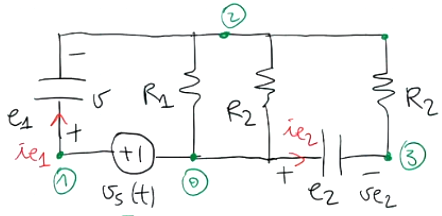
\includegraphics[width = 0.4\linewidth]{circuito_esercizio_1}
\end{figure}
$$
R_1 = \SI{2}{\ohm}\ \ R_2 = \SI{3}{\ohm}\ \ C_1 = \SI{3}{\farad}\ \ C_2 = \SI{1}{\farad}
$$
Per determinare le equazioni di stato si sostituisce il circuito con il circuito
resistivo associato, sostituendo ad ogni condensatore un generatore di tensione
equivalente e calcolando in seguito le correnti $i_{C_1}$ e $i_{C_2}$.
Sostituiti i condensatori si calcolano le correnti con il PSE.

Il primo circuito chiamato $C'$ ha solo la tensione $v_{C_1}$ diversa da zero
mentre gli altri generatori sono spenti (cortocircuiti), il circuito $C''$ ha il generatore $v_{C_2}$ attivo, il circuito $C'''$ ha il generatore $v_s$ attivo.

$$
\begin{aligned}
C' & \\
R_{eq} &= (R_1//R_2)//R_2\\
i_{C_1'} &= - \frac{V_{C_1}}{R_{eq}} \\
i_{C_2'} &= \frac{V_{C_1}}{R_2}
\end{aligned}
\qquad
\begin{aligned}
C'' & \\
i_{C_1'} &= \frac{V_{C_2}}{R_2}\\
i_{C_2'} &= -\frac{V_{C_2}}{R_2}
\end{aligned}
\qquad
\begin{aligned}
C''' & \\
i_{C_1'''} &= \frac{V_s}{R_{eq}} \\
i_{C_2'''} &= -\frac{V_s}{R_2}
\end{aligned}
$$
Si può ora applicare il principio di sovrapposizione degli effetti
sommando i vari contributi
$$
\begin{aligned}
i_{C_1} & = -\frac{V_{C_1}}{R_{eq}} + \frac{V_{C_2}}{R_2} + \frac{V_s}{R_{eq}} =
C_1\frac{dv_{C_1}}{dt}\\
i_{C_2} & = -\frac{V_{C_1}}{R_2} - \frac{V_{C_2}}{R_2} - \frac{V_s}{R_2} =
C_2\frac{dv_{C_2}}{dt}
\end{aligned}
$$
\subparagraph{2.a) Risposta all'impulso con C.I.}
Si determina ora la risposta impulsiva con il metodo delle condizioni iniziali con 
generatore impulsivo.
Si sostituiscono ancora una volta i bipoli dinamici con corto circuiti o circuiti
aperti (nel caso in cui siano condensatori o induttori) e si impone il generatore
$V_s(t) = \delta(t)$ ricordando che $R_{eq}=\frac{6}{7}\si{\ohm}$
\begin{align*}
i_{C_1} &= \frac{\delta(t)}{R_{eq}} = \frac{7}{6}\delta(t)\\
i_{C_2} &= -\frac{\delta(t)}{R_2} = -\frac{1}{3}\delta(t)
\end{align*}

Sostituendo con la caratteristica del condensatore e integrando si ha
\begin{align*}
\left(V_{C_1}(0^-) = \SI{0}{\volt}\right)\ \ C_1V_{C_1}(0^+) &=\int_{0^-}^{0^+}C_1\frac{dV_{C_1}}{dt}dt = \int_{0^-}^{0^+}\frac{7}{6}\delta(t)dt = \frac{7}{6} \Rightarrow V_{C_1}(0^+) = \frac{7}{18}\si{\volt}\\
\left(V_{C_2}(0^-) = \SI{0}{\volt}\right)\ \ C_2V_{C_2}(0^+) & = \int_{0^-}^{0^+} C_2 \frac{dV_{C_2}}{dt}dt =
\int_{0^-}^{0^+} -\frac{1}{3}\delta(t) dt = -\frac{1}{3} \Rightarrow V_{C_2}(0^+) = -\frac{1}{3}\si{\volt}
\end{align*}
Determinate le condizioni iniziali si sa che la soluzione del circuito è proprio
l'evoluzione libera, con generatore spento a partire da queste condizioni iniziali.

Si vuole ricavare la $V_{C_1}$, si ricava quindi $V_{C_2}$ dalla prima equazione di stato in funzione della $V_{C_1}$ e la si sostituisce nella seconda.
$$
V_{C_2} = R_2 \left( \frac{V_{C_1}}{R_{eq}} + C_1\frac{dV_{C_1}}{dt} \right)
$$
$$
\frac{V_{C_1}}{R_2} - \frac{V_{C_1}}{R_{eq}} - C_1\frac{dV_{C_1}}{dt} - \cancel{\frac{V_s}{R_2}} = 
C_2\left(\frac{R_2}{R_{eq}}\frac{dV_{C_1}}{dt} + R_2C_1\frac{d^2V_{C_1}}{dt^2}\right)
$$
$$
C_2C_1R_2\frac{d^2V_{C_1}}{dt^2} + \left(\frac{C_2R_2}{R_{eq}}+C_1\right)\frac{dV_{C_1}}{dt} +
\left(\frac{1}{R_{eq}}-\frac{1}{R_2}\right)V_{C_1} = 0
$$
Per verificare la correttezza dei calcoli si nota che dimensionalmente tutti i termini 
hanno sono la stessa grandezza (in questo caso la corrente) e che il segno dei coefficienti
sia concorde affinché la grandezza in esame nel circuito dissipativo si smorzi nel tempo.

Per trovare le radici del polinomio caratteristico è utile rendere unitario il coefficiente del
termine di grado più elevato.
$$
\lambda^2 + \left(\frac{1}{R_{eq}C_1} + \frac{1}{R_2C_2}\right)\lambda + \left(\frac{1}{R_{eq}}-\frac{1}{R_2}\right)\frac{1}{C_2C_1R_2} = 0
$$
$$
\lambda^2+\frac{13}{18}\lambda + \frac{5}{54} = 0
$$
Si calcolano dunque le radici:
$$
\lambda_{1,2} = -\frac{13}{36} \pm \sqrt{\left(\frac{13}{36}\right)^2-\frac{5}{54}} = 
\begin{cases}
\lambda_1 = -0.556\\
\lambda_2 = -0.167
\end{cases}
$$
La soluzione sarà del tipo
$$
V_{C_1}(t) = K_1 e^{-0.556 t} + K_2 e^{-0.167 t}
$$
\newpage
Si ricavano le costanti $K_1$ e $K_2$ mediante le condizioni iniziali prima ricavate.

$$
\begin{aligned}
V_{C_1}(0^+) &= \frac{7}{18} = K_1 + K_2 \\
\frac{dV_{C_1}}{dt}(0^+) &= -0.188 = \lambda_1K_1 + \lambda_2K_2
\end{aligned}
\Rightarrow
\begin{cases}
K_2 = 0.0714\\
K_1 = 0.3175
\end{cases}
$$
Assemblando il risultato si ottiene:
$$
V_{C_1}(t) = h(t) = 0.3175e^{-0.556 t} + 0.0714 e ^{-0.617 t}, \ \ t\geq 0
$$

\subparagraph{2.b) Modo alternativo con risposta al gradino}
Ricordando che nei punti regolari o nel senso delle distribuzioni $h(t) = \frac{dg}{dt}$.
Il gradino è una soluzione a regime, quindi si può recuperare il risultato precedente
e aggiungere la soluzione di regime.
Si sostituiscono nel circuito i condensatori con circuiti aperti
\begin{figure}[H]
\centering
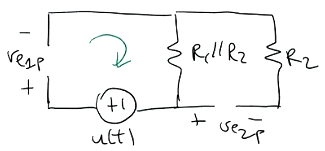
\includegraphics[width=0.6\linewidth]{circuito_esercizio_1_regime}
\end{figure}
$$
V_{C_{1p}} = u(t)
$$
$$
g(t) = K_1'e^{-0.556t} + K_2'e^{-0.167 t} + u(t)
$$
Ricordando che $u(t)=1,\ t>0$ si ricavano le nuove condizioni iniziali per determinare
i coefficienti $K_1'$ e $K_2'$
$$
\begin{aligned}
g(0^+) &= K_1' + K_2' + 1 = 0\\
\frac{dg}{dt}(0^+) &= \frac{1}{R_{eq}C_1} = \frac{7}{18}
\end{aligned}
\Rightarrow
\begin{aligned}
K_1' = -0.5704 \\
K_2' = -0.4296
\end{aligned}
$$
La risposta al gradino è dunque:
$$
g(t) = V_{C_1}(t) = -0.5704 e^{-0.556t} - 0.4296e^{-0.167t} + 1,\ t\geq 0
$$
$$
h(t) = \frac{dg}{dt} = 0.3175e^{-0.556t}+0.0714e^{-0.167 t},\ t\geq 0
$$
1:16:46
